\ifx \globalmark \undefined %% This is default.
	\documentclass[twoside,openright,11pt,a4paper]{report}

%\compiler avec xelatex
%\usepackage[applemac]{inputenc}
\usepackage[T1]{fontenc}
\usepackage[utf8]{inputenc} %latin1 est possible
%\usepackage[latin1]{inputenc} %latin1 est possible
\usepackage[UKenglish]{babel}
\usepackage{lettrine}

%\usepackage[text={13cm,20cm},centering]{geometry}
\usepackage [squaren, Gray, mediumqspace]{SIunits}
\usepackage [top=2cm, bottom=2cm, left=2cm, right=2cm ]{geometry}

\renewcommand{\familydefault}{cmss}
\addto\captionsenglish{ \renewcommand\chaptername{Solutions of Chapte}}

\usepackage{graphicx}
\usepackage{amsmath}
\usepackage{amsfonts}
\usepackage{amssymb}
\usepackage{amsthm}
\usepackage{bm}
\usepackage{color}

\newcommand{\real}{\mathbb{R}}
\newcommand{\mb}{\mathbf}
\newcommand{\bos}{\boldsymbol}

\def \RR {I \! \! R}

\newcommand{\e}{\begin{equation}}  
\newcommand{\ee}{\end{equation}}
\newcommand{\eqn}{\begin{eqnarray}} 
\newcommand{\eeqn}{\end{eqnarray}} 
\newcommand{\eqnn}{\begin{eqnarray*}} 
\newcommand{\eeqnn}{\end{eqnarray*}} 

\newcommand{\bpm}{\begin{pmatrix}}
\newcommand{\epm}{\end{pmatrix}}

%\newcommand{\{\c c}}{\c c}

\newcommand{\bma}{\left(\begin{array}}
\newcommand{\ema}{\end{array}\right)} 
\newcommand{\hh}{\hspace{2mm}}
\newcommand{\hd}{\hspace{5mm}}
\newcommand{\hu}{\hspace{1cm}}
\newcommand{\vv}{\vspace{2mm}}
\newcommand{\vd}{\vspace{5mm}}
\newcommand{\vm}{\vspace{-2mm}}
\newcommand{\teq}{\triangleq}
%\newcommand{\qedb}{\,$\Box$}
\newcommand{\blanc}{$\left. \right.$}
\newcommand{\frts}[2]%
         {\frac{{\textstyle #1}}{{\textstyle #2}}}

\newcommand{\bindex}[3]%
{
\renewcommand{\arraystretch}{0.5}
\begin{array}[t]{c}
#1\\
{\scriptstyle #2}\\
{\scriptstyle #3}
\end{array}
\renewcommand{\arraystretch}{1}
}

\theoremstyle{definition}
\newtheorem{exemple}{{\bf Exemple}}[chapter]
\newtheorem{theoreme}[exemple]{{\bf Th{é}or{è}me}}
\newtheorem{propriete}[exemple]{{\bf Propri{é}t{é}}}
\newtheorem{definition}[exemple]{{\bf D{é}finition}}
\newtheorem{remarque}[exemple]{{\bf Remarque}}
\newtheorem{remarques}[exemple]{{\bf Remarques}}
\newtheorem{lemme}[exemple]{{\bf Lemme}}
\newtheorem{hypothese}[exemple]{{\bf Hypoth{è}se}}
\newtheorem{exercice}{{\bf Exercice}}[chapter]

\newcommand{\xqedhere}[2]{%
 \rlap{\hbox to#1{\hfil\llap{\ensuremath{#2}}}}}

\newcommand{\xqed}[1]{%
 \leavevmode\unskip\penalty9999 \hbox{}\nobreak\hfill
 \quad\hbox{\ensuremath{#1}}}

\newcommand{\gf}{\fg\,\,}

\newcommand{\cata}[1] %
     {\renewcommand{\arraystretch}{0.5}
     \begin{array}[t]{c} \longrightarrow \\ {#1} \end{array}
     \renewcommand{\arraystretch}{1}}

\usepackage[isu]{caption}
%\usepackage[font=small,format=plain,labelfont=bf,up,textfont=it,up]{caption}
\setlength{\captionmargin}{60pt}

\newcommand{\cqfd}
{%
\mbox{}%
\nolinebreak%
\hfill%
\rule{2mm}{2mm}%
\medbreak%
\par%
}

\pagestyle{headings}

\renewcommand{\sectionmark}[1]{%
\markright{\thesection.\ #1}{}}

\renewcommand{\chaptermark}[1]{%
\markboth{\chaptername\ \thechapter.\ #1}{}}

\makeatletter 
\def\@seccntformat#1{\csname the#1\endcsname.\;} 
\makeatother

\title{ {\Huge {\textbf{Modélisation et analyse  \\ \vspace{4mm} des systèmes dynamiques }}} \\ \vspace{4cm} G. Bastin}

%\title{ {\Huge {\textbf{Modelisation et analyse  \\ \vspace{4mm} des systemes dynamiques }}} \\ \vspace{4cm} G. Bastin}


\date{\today}
	\begin{document} %% Crashes if put after (one of the many mysteries of LaTeX?).
\else 
	\documentclass{standalone}
	\begin{document}
\fi

\graphicspath{ {Chapitre4/images/} }

\setcounter{chapter}{3}
\chapter{Systèmes à compartiments}
\chaptermark{Systèmes à compartiments}\label{syscompart}


\lettrine[lines=1]{\bf L}{}a notion de système à compartiments est utilisée pour désigner une 
vaste classe de systèmes dont la 
dynamique peut être décrite par des équations de  bilan.
Elle trouve des applications dans de nombreux domaines des sciences
de l'ingénieur (tels que le génie chimique, le génie biomédical
 ou l'écologie) mais aussi en sciences économiques et sociales.

\section{Définitions et notations}

Un compartiment est un réservoir conceptuel dont le contenu (matière,
énergie, monnaie, population ...) est quantifiable. On utilise la représentation 
symbolique indiquée à la figure \ref{fig:compartiment} où $q_{in}$ et
$q_{out}$ indiquent, respectivement, les flux d'alimentation et de vidange
du compartiment exprimés en quantité de contenu par unité de temps.
Ces flux sont toujours {\em positifs} par convention.

\begin{figure}[ht]
\begin{center}
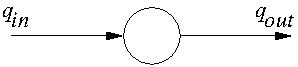
\includegraphics{compartiment}
\caption{Représentation symbolique d'un compartiment}
\label{fig:compartiment}
\end{center}
\end{figure}

Un système à compartiments est constitué par un {\em réseau} de 
compartiments interconnectés et numérotés de $1$ à $n$. Pour fixer
les idées, un exemple de système à $3$ compartiments est représenté
à la figure \ref{fig:exemplecomp}. Les flèches indiquent les flux de
contenu que les divers compartiments peuvent échanger entre eux et avec
l'extérieur du système.

\begin{figure}[ht]
\begin{center}
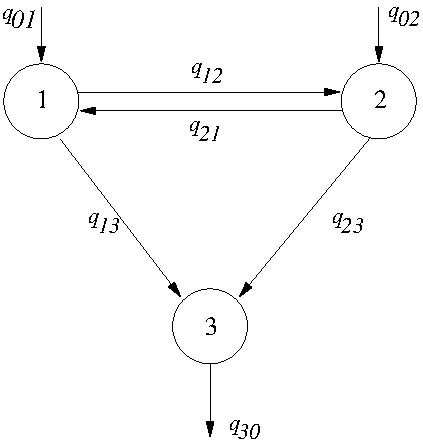
\includegraphics[width=5cm]{exemplecomp}
\caption{Exemple de graphe d'un système à compartiments}
\label{fig:exemplecomp}
\end{center} 
\end{figure}

D'une manière générale, un système à compartiments sera donc 
représenté par un {\em graphe orienté} dont les noeuds correspondent 
aux compartiments et les arcs aux flux. On introduit les notations suivantes~:
\begin{description}
\item $x_i$ désigne la quantité contenue dans le compartiment d'indice $i$,
$(i = 1, ... ,n)$. Cette quantité est toujours {\em positive}. Avec un léger
abus de langage, on
dira aussi pour simplifier que $x_i$ désigne le {\em niveau} du compartiment $i$.
\item $q_{ij}$ désigne le flux circulant du compartiment $i$ vers 
le compartiment $j$, $(i = 1, ... ,n ; j = 1, ... ,n)$. Comme nous l'avons indiqué 
plus haut, c'est une variable qui est aussi toujours {\em positive} par convention.
\end{description}

\begin{definition}{\bf \em Système ouvert ou fermé}

On dit que le système est {\bf ouvert} lorsqu'il existe des possibilités 
d'échange avec l'extérieur du système. Dans ce cas :
\begin{description}
\item $q_{io}$ désigne le flux circulant du compartiment $i$ vers l'extérieur
\item $q_{oi}$ désigne le flux circulant de l'extérieur vers le compartiment $i$
\end{description}
Dans le cas contraire, on dit que le système est {\bf fermé} : $q_{io} = 
q_{oi} = 0$ pour tout $i$. \qed
\end{definition}

\begin{definition}{\bf \em Système connecté aux entrées et sorties}

Un compartiment $i$ est {\it connecté à une sortie} si il y a un chemin $i \rightarrow j \rightarrow k \rightarrow \dots \rightarrow \ell$ partant de ce compartiment et se terminant en un compartiment $\ell$ à partir duquel il y a un flux de sortie $q_{\ell o}$. Le système est {\it complètement connecté aux sorties} (CCS) si chaque compartiment est connecté à une sortie.

Un compartiment $\ell$ est {\it connecté à une entrée} si il y a un chemin $i \rightarrow j \rightarrow k \rightarrow \dots \rightarrow \ell$ jusqu'à ce compartiment et partant d'un compartiment $i$ dans lequel il y a un flux d'entrée $q_{oi}$. Le système est {\it complètement connecté aux entrées} (CCE) si chaque compartiment est connecté à une entrée.  \qed 
\end{definition}


\section{Modèle d'état}
\markboth{ {\bf \hspace*{5mm}Chapitre 4 }\hfill Systèmes
à compartiments} {{ \bf Sec. \thesection} \hfill
Modèles d'état \hspace*{5mm}}

L'équation de bilan de chaque compartiment (appelée aussi équation de
continuité)
\eqnn
\dot{x_i} = \sum_{j=0}^n q_{ji}(t) - \sum_{j=0}^n q_{ij}(t) \hspace{1cm} i=1,...,n
\label{bilan}
\eeqnn
est l'élément de base pour l'établissement du modèle d'état d'un système
à compartiments. Cette équation exprime que la variation, par 
unité de temps,  de la 
quantité contenue dans un
compartiment est la différence entre la somme des
flux (ou débits) entrants et la somme des flux (ou débits) 
sortants. En pratique, bien s\^ur, les flux qui sont structurellement nuls 
ne sont pas explicités dans l'équation (\ref{bilan}).

La mise en équations du modèle d'état d'un système à compartiments
comporte dès lors deux aspects fondamentaux.

Tout d'abord, la structure du graphe associé au système détermine le nombre
et la structure des équations de bilan (\ref{bilan}) ; les variables $x_i$ sont
les variables d'état tandis que l'ordre du modèle est le nombre $n$ de 
compartiments.

Pour compléter le modèle d'état, il faut ensuite exprimer les flux
en fonction des variables d'état et des variables d'entrée :
\eqnn
q_{ij}(x,u)
\eeqnn
où $x$ et $u$ désignent, comme d'habitude, les vecteurs d'état et 
d'entrée. Cette modélisation fera l'objet de la prochaine section.

La forme générale des équations d'état d'un système à compartiments
est alors la suivante :
\eqnn
\dot{x_i} = \sum_{j=0}^n q_{ji}(x,u) - \sum_{j=0}^n q_{ij}(x,u) \hspace{1cm} i=1,...,n \label{eqetcomp}
\eeqnn
Dans ce modèle, le sens physique des variables d'état $x_i$ est clair : ce sont
les quantités contenues dans chaque compartiment. Par contre, les variables
d'entrée $u$ peuvent être de nature très variable selon les applications comme le montreront les exemples qui vont suivre.

Si l'on définit le {\em vecteur des flux} $q(x,u)$ contenant, dans un ordre arbitraire, 
tous les flux $q_{ij}(x,u)$
qui ne sont pas structurellement nuls, on peut écrire aussi le modéle d'état
(\ref{eqetcomp}) sous la forme matricielle plus compacte :
\eqn
\dot{x} = Lq(x,u) \label{modetcomp}
\eeqn
où $L$ est la matrice d'incidence du graphe orienté, dont les coefficients appartiennent tous au triplet
$(-1,0,1)$, qui est .

\begin{exemple}
Pour le système représenté à la figure \ref{fig:exemplecomp}, le
modèle d'état s'écrit :
\eqnn
\dot{x_1} &=& q_{01}(x,u) - q_{12}(x,u) - q_{13}(x,u) + q_{21}(x,u) \\
\dot{x_2} &=& q_{02}(x,u) + q_{12}(x,u) - q_{21}(x,u) - q_{23}(x,u) \\
\dot{x_3} &=& q_{13}(x,u) + q_{23}(x,u) - q_{30}(x,u)
\eeqnn
Si l'on définit le vecteur des flux :
\eqnn
q(x,u) \triangleq \bma{c} q_{01}(x,u) \\ q_{02}(x,u) \\ q_{12}(x,u) \\
q_{13}(x,u) \\ q_{21}(x,u) \\ q_{23}(x,u) \\ q_{30}(x,u) \ema
\eeqnn
le modèle d'état s'écrit sous la forme matricielle (\ref{modetcomp}) avec 
la matrice $L$ :
\eqnn
L \triangleq \bma{ccccccc} 1 & 0 & -1 & -1 & 1 & 0 & 0 \\
0 & 1 & 1 & 0 & -1 & -1 & 0 \\
0 & 0 & 0 & 1 & 0 & 1 & -1 \ema.
\eeqnn
\qed
\end{exemple}

\section{Modélisation des flux}

Selon les applications, les fonctions $q_{ij}(x,u)$ représentant les flux peuvent prendre des formes très variées.  Elles doivent cependant être définies de manière à garantir que le système à compartiments est un {\em système positif} c'est à dire un système dont chaque variable
d'état reste positive le long des trajectoires. C'est une garantie de vraisemblance du modèle puisque les variables d'état représentent des grandeurs qui n'ont pas de sens physique si
elles sont négatives.

\begin{definition} \label{vecpositif} {\bf \em Vecteur positif et orthant positif}

Un vecteur $x = (x_1, \ldots , x_n)^T$ est positif (notation
$x \geq 0$) si chacune de ses composantes est un nombre réel positif~:
$x_i \geq 0$ pour tout $i$.

L'orthant positif de dimension $n$ (noté $\RR_+^n$) est l'ensemble de tous les vecteurs positifs de dimension $n$. \qed
\end{definition}

\begin{definition}{\bf \em Système positif}

Un système dynamique $\dot x=f(x,u)$ est un système positif si, pour toute entrée $u(t)$ admissible, son état
est confiné dans l'orthant positif lorsque l'état initial est positif~:
\eqnn
x(t_0) \in \real_+^n \text{ et } u(t) \in {\cal U}  \Longrightarrow x(t)
\in \real_+^n  \hh \forall t \geq t_0. \qed
\eeqnn
\end{definition}

Le théorème suivant donne une condition suffisante facile à utiliser pour vérifier qu'un système est positif. 

\begin{theoreme} 
Un système dynamique $\dot x=f(x,u)$ est un système positif si $f(x,u)$ est différentiable et si
\eqnn
x \in \real_+^n \;\;\;\; \mbox{et} \;\;\;\; x_i = 0 \;\; \Longrightarrow \;\; \dot x_i \geq 0 \;\;\;\; \forall i. \qed
\eeqnn
\end{theoreme}
Pour garantir qu'un système à compartiments est un système positif, on impose les conditions suivantes aux fonctions de flux $q_{ij}(x,u)$~:
\begin{itemize}
\item[C1.]  Les fonctions $q_{ij}(x,u)$ sont des fonctions positives de leurs arguments sur leur domaine de définition~:
\eqnn
q_{ij}(x,u) : \real^n_+ \times \real^m \rightarrow \real_+
\eeqnn 
\item[C2.] Les fonctions $q_{ij}(x,u)$ sont des fonctions continues et dérivables de leurs arguments sur leur domaine de définition.
\item[C3.]  Comme il ne peut y avoir de flux sortant d'un compartiment vide, les fonctions $q_{ij}(x,u)$ vérifient la condition~:
\eqnn
x_i = 0 \;\; \Rightarrow \;\; q_{ij}(x,u) = 0
\eeqnn
\end{itemize}


\begin{theoreme}
Sous les conditions C1, C2, C3, un système à compartiments $\dot x = Lq(x,u)$
est un système positif.
\cqfd
\end{theoreme}
\begin{exemple}\label{systhyd}{\bf \em Système hydraulique}

Considérons un système hydraulique formé d'un ensemble 
de réservoirs situés à des altitudes différentes
et dont le contenu liquide s'écoule \og en cascade \gf
des réservoirs les plus élevés vers les réservoirs les plus bas sous l'action
de la gravité. Un exemple est illustré à la figure \ref{Fig:cascade}.
\begin{figure}[h] 
\begin{center}
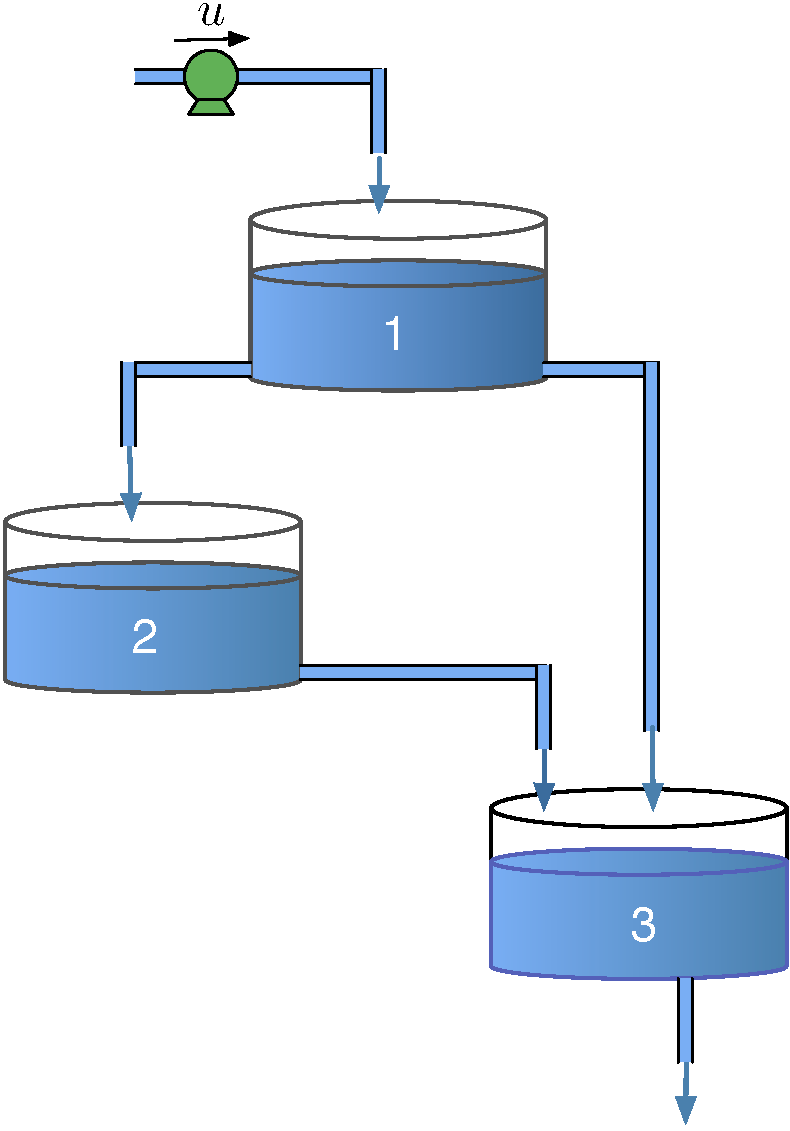
\includegraphics[width=7cm]{cascade}
\caption{Cascade de réservoirs}
\label{Fig:cascade}
\end{center} 
\end{figure}

Il s'agit clairement d'un système à compartiments dont le graphe associé
est représenté à la figure \ref{Fig:grafassoc} et dont les équations de 
continuité s'écrivent~:
\begin{equation*} \begin{split} 
\dot x_1 &= q_{01} - q_{12} - q_{13} \\
\dot x_2 &=  q_{12} - q_{23} \\
\dot x_3 &= q_{13} + q_{23} - q_{30} 
\end{split} \end{equation*}
\begin{figure}[h] 
\begin{center}
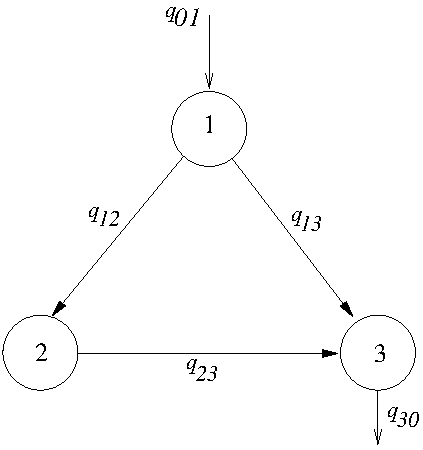
\includegraphics[width=7cm]{grafassoc}
\caption{Graphe associé à la cascade de résevoirs}
\label{Fig:grafassoc}
\end{center} 
\end{figure}
Dans ces équations, les variables d'état $x_1$,$ x_2$ et $x_3$ désignent 
évidemment les volumes d'eau contenus dans les réservoirs et les flux 
$q_{ij}$ représentent les débits s'écoulant des réservoirs supérieurs
vers les réservoirs inférieurs. Pour compléter le modèle, il faut 
exprimer ces flux en fonction des variables d'état et de signaux d'entrée
convenablement choisis.
Le débit fourni par la
pompe d'alimentation du réservoir supérieur peut clairement être choisi
comme variable d'entrée. Le débit de sortie $q_{ij}$
de chaque réservoir est une fonction positive du volume $x_i$ du réservoir. La forme de cette fonction dépend de la forme du réservoir et de la configuration de l'orifice par lequel l'eau s'écoule. Considérons le cas où les réservoirs sont de section horizontale constante et où l'écoulement s'effectue par un orifice rectangulaire situé au bas des réservoirs. La hauteur de l'eau dans un réservoir est notée~:
\eqnn
h_i = \frac {x_i}{S_i}
\eeqnn
où $S_{i}$ désigne la section du réservoir.
Selon les lois de l'hydraulique, nous savons que, lorsque la hauteur de l'eau $h_i$ est grande par rapport à la hauteur de l'orifice, la relation entre le débit et la hauteur d'eau est proportionnelle à $\sqrt{h_i}$ (loi de Torricelli~\footnote{Cette loi énoncée par Torricelli en 1643 énonce que la vitesse $v$ de l'eau à la sortie d'un réservoir de hauteur $h$ vérifie $v^2=2gh$. Elle se démontre intuitivement par analogie avec un corps en chute libre: un volume élémentaire d'eau à la surface du réservoir transforme son énergie potentielle $\rho g h$ en énergie cinétique $\rho v^2/2$ quand il arrive à la sortie du réservoir, où $\rho$ désigne la masse volumique. Plus rigoureusement, on la déduit du théorème de Bernoulli sans perte de charge ou pompe $p+\rho gz +\rho v^2/2 = \mathrm{constante}$, où $p$ désigne la pression et $z$ l'altitude.}). Par contre lorsque la hauteur de l'eau est inférieure à la hauteur de l'orifice, le débit devient proportionnel à $h_i\sqrt{h_i}$ (loi de l'écoulement pour un déversoir de forme rectangulaire). On peut dès lors proposer un modèle de la forme~:
\eqnn
q_{ij} = \frac { \alpha_{ij}h_i\sqrt{h_i} }{ \beta_{ij} + h_i}
\eeqnn
où $ \alpha_{ij}$ et $ \beta_{ij}$ sont des constantes positives. En effet ce modèle vérifie bien la propriété que pour de faibles hauteurs d'eau ($h_i \ll \beta_{ij}$), le débit $q_{ij}$ est proportionnel à $h_i\sqrt{h_i}$ tandis que pour des hauteurs d'eau élevées ($h_i \gg \beta_{ij}$), le débit $q_{ij}$ est proportionnel à $\sqrt{h_i}$.
On peut exprimer $q_{ij}$ en fonction de $x_i$~:
\eqnn
q_{ij}(x_i) = \frac {k_{ij}x_i\sqrt{x_i} }{S_i \beta_{ij} + x_i} \hh \mbox{ avec } k_{ij} \triangleq \frac{\alpha_{ij}}{\sqrt{S_i}} 
\eeqnn
Alors le modèle d'état s'écrit finalement~:
\begin{equation} \begin{split} \label{modetacasca}
\dot x_1 &= - \frac {k_{12}x_1\sqrt{x_1} }{S_1\beta_{12} + x_1} - \frac {k_{13}x_1\sqrt{x_1} }{S_1 \beta_{13} + x_1} + u, \\
\dot x_2 &=  \frac {k_{12}x_1\sqrt{x_1} }{S_1 \beta_{12} + x_1} - \frac {k_{23}x_2\sqrt{x_2} }{S_2 \beta_{23} + x_2},
\\
\dot x_3 &= \frac{k_{13}x_1\sqrt{x_1} }{S_1 \beta_{13} + x_1} + \frac {k_{23}x_2\sqrt{x_2} }{S_2 \beta_{23} + x_2} -
\frac {k_{30}x_3\sqrt{x_3} }{S_3 \beta_{30} + x_3}.
\end{split} \end{equation}
On observe que les fonctions $q_{ij}(x_{i})$ vérifient bien les conditions de positivité C1, C2, C3. \qed
\end{exemple}


%%%%%%%%%%%%%%%%%%%%%%%%%%%%%%%%%%%%%%%%%%%%%%%%%%
%%%%%%%%%%%%%%%%%%%%%%%%%%%%%%%%%%%%%%%%%%%%%%%%%%
%%%%%%%%%%%%%%%%%%%%%%%%%%%%%%%%%%%%%%%%%%%%%%%%%%
%%%%%%% PARTIE DE DOUNIA MULDERS    %%%%%%%%%%%%%%
%%%%%%%%%%%%%%%%%%%%%%%%%%%%%%%%%%%%%%%%%%%%%%%%%%
%%%%%%%%%%%%%%%%%%%%%%%%%%%%%%%%%%%%%%%%%%%%%%%%%%
%%%%%%%%%%%%%%%%%%%%%%%%%%%%%%%%%%%%%%%%%%%%%%%%%%


\section{Linear models driven by controlled external supplies}

This is the most represented class of compartmental models within the literature.
It is characterized by the following flow definitions:
\begin{enumerate}
\item Flows between compartments and system output flows  are linear in function of the providing compartment level:
\eqnn
q_{ij} = k_{ij}x_i \hspace{1cm} k_{ij} > 0 \hspace{1cm} (i=1,...,n;j=0,...,n)
\eeqnn
\item The system inputs $u_{\ell}$ are proportional to the supply flow: 
\eqnn
q_{0\ell} = k_{0\ell}u_{\ell} 
\eeqnn
\end{enumerate}

In that case, the required information used to write the state model is entirely unclosed within the system graph.
The state model can be represented as a linear system (see chapter 1):
\eqnn
\dot{x} = Ax + Bu
\eeqnn
with the following structural features:
\begin{enumerate}
\item Matrix $A$ is a {\em Metzler matrix} i.e. such that $a_{ij} \geq 0$ for all $i \neq j$
\item Matrix $A$ is diagonally dominant i.e.
\eqnn |a_{ii}| \geq \sum_{j \neq i} a_{ji} 
\eeqnn
\item Matrix $B$ is a full rank {\em elementary matrix}, i.e. a matrix containing at most one non null element per line and per column.
\end{enumerate}

\begin{exemple}
The compartmental system linear state model corresponds to the graph shown on \ref{fig:exemplecomp} 
and can be written as:
\begin{equation} \begin{split}
\bma{c} \dot x_1 \\ \dot x_2 \\ \dot x_3 \ema &= 
\bma{ccc} -(k_{12} + k_{13}) & k_{21} & 0 \\ 
k_{12} & -(k_{21} + k_{23}) & 0 \\ k_{13} & k_{23} & - k_{30} \ema
\bma{c} x_1 \\ x_2 \\ x_3 \ema \\ &\hd
+ \bma{cc} k_{01} & 0 \\ 0 & k_{02} \\ 0 & 0 \ema
\bma{c} u_1 \\ u_2 \ema
\end{split} \end{equation}
We observe that $A$ is a diagonally dominant Metzler matrix and that $B$ is a full rank elementary matrix ($rank = 2$).
\cqfd
\end{exemple}

\begin{exemple}{\bf \em Physiological modelling}
Physiologists are often interested in describing and analyzing biological or chemical substance propagation within mammal body.
Those substances can stand for medicinal substances (Pharmacokinetic studies) or toxic substances voluntary or accidentally absorbed.
They can also be natural substances such as hormones or proteins.
Compartmental models are frequently used to process such studies: 
the mammal body is therefore represented as a more or less diversified group of interconnected vessels.

Let us consider the example on figure \ref{Fig:grapharmaco}.
\begin{figure}[ht] 
\begin{center}
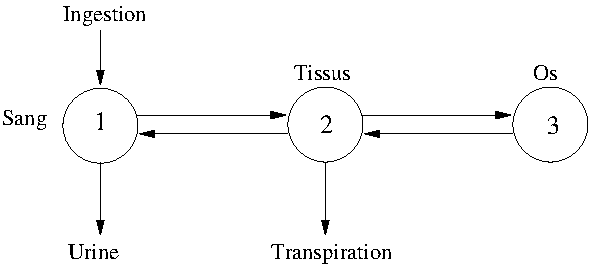
\includegraphics{grapharmaco}
\caption{Pharmacokinetic compartmental graph model}
\label{Fig:grapharmaco}
\end{center} 
\end{figure}

A toxic substance (lead for example) is absorbed by an animal and permeated in its blood.
This substance progressively propagates within the body, from the blood to tissues at first, towards bones afterwards.
It is secreted by sweating from one part and by urinating from the other part.
The linear compartmental model corresponding to the graph on figure \ref{Fig:grapharmaco} is the following model:
\begin{equation*} \begin{split}
\bma{c} \dot x_1 \\ \dot x_2 \\ \dot x_3 \ema &= 
\bma{ccc} -(k_{10} + k_{12}) & k_{21} & 0 \\ 
k_{12} & -(k_{20} + k_{21} + k_{23}) & k_{32} \\ 0 & k_{23} & - k_{32} \ema
\bma{c} x_1 \\ x_2 \\ x_3 \ema \\
& \hd + \bma{c} k_{ 01}\\ 0 \\ 0 \ema u.
\end{split} \end{equation*}
In this model, the state variables are: $x_1$, $x_2$ et $x_3$, which stands for toxial substance quantities within the three compartments (blood, tissues and bones).
The input variable $u$ stands for the body ingestion flow.
\cqfd
\end{exemple}


\section{Non linear model with controlled flows}
We will now consider non linear compartmental systems which flows $q_{ij}$ can be non linear functions whose arguments respect the C1 - C3 conditions.
We already approached a non linear model in the vessels cascade example.
However, flows between compartments were not depending on input variables $u_{\ell}$ in that example.
We will here consider a case where flows between compartments are explicit functions of input variables $u_{\ell}$ 
allowing to monitor the debit between compartments.
The symbolic representation presented on figure \ref{Fig:contflux} shows the presence of such a monitoring variable.
\begin{figure}[ht] 
\begin{center}
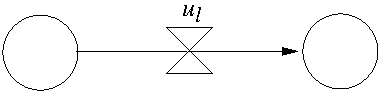
\includegraphics{contflux}
\caption{Symbolic representation of a monitored flow}
\label{Fig:contflux}
\end{center} 
\end{figure}


\begin{exemple}{\bf \em Vessels network}
Let us consider the hydraulic system represented on figure \ref{Fig:reseauh}. 
This vessels network corresponds to the vessel cascade example (\ref{systhyd} with a small modification:
the flow between vessel $2$ and vessel $3$ is now monitored by a pump.
As this pump is controllable, we can consider the pumped debit $F$ as an input variable.

\begin{figure}[h] 
\begin{center}
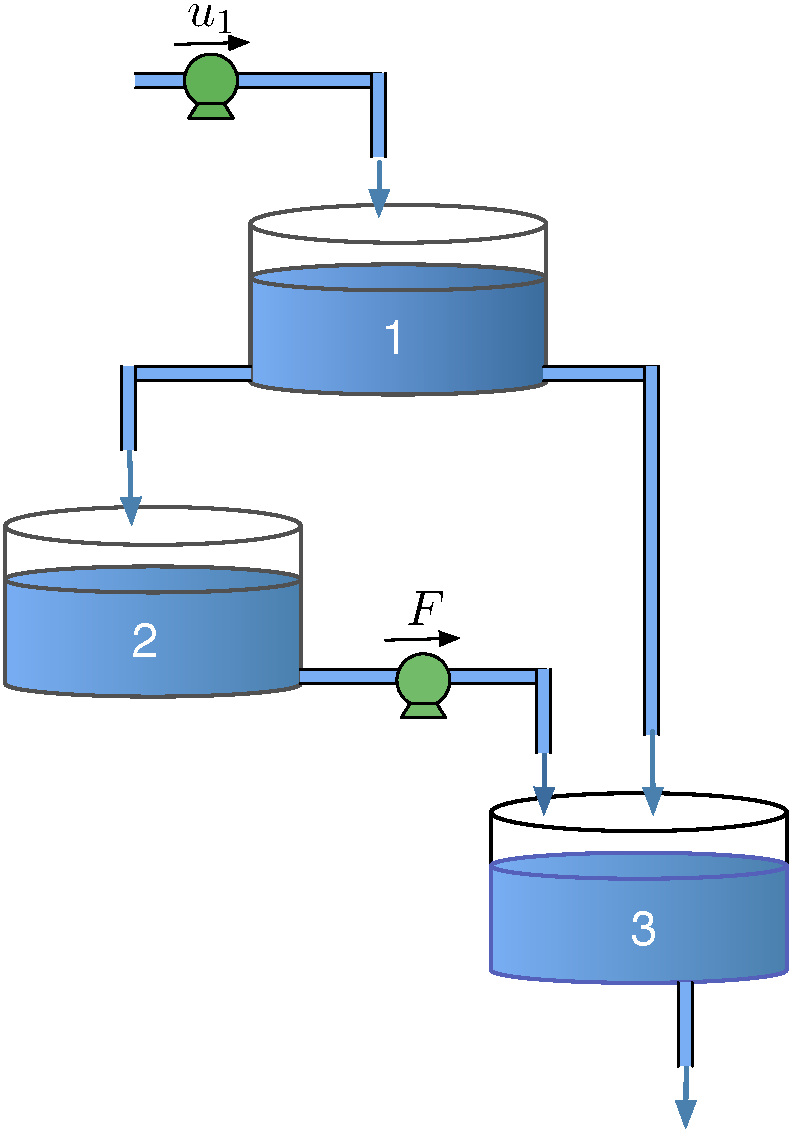
\includegraphics[width=7cm]{reseauh}
\caption{Vessels networks}
\label{Fig:reseauh}
\end{center} 
\end{figure}

The state model (\ref{modetacasca}) we obtained for the vessels cascade is therefore simply modified as follows:
\begin{equation} \begin{split}
\dot x_1 &= - q_{12}(x_1) - q_{13}(x_1) + u_1 \\
\dot x_2 &=  q_{12}(x_1) - u_2 \label{modres1} \\
\dot x_3 &= q_{13}(x_1) - q_{30}(x_3) + u_2 
\end{split} \end{equation}
where the state variables $x_i$ stand for water volumes contained in vessels,
input variable $u_1$ corresponds to the first vessel supply debit,
input variable $u_2 = F$ corresponds to the pumped flow from the second vessel towards the third vessel
and functions $q_{ij}(x_i)$ are defined as follows:
\eqnn
q_{ij}(x_i) = \frac {k_{ij}x_i\sqrt{x_i} }{S_i \beta_{ij} + x_i}
\eeqnn
We observe that this state model {\it cannot} represents a compartmental system respecting C1-C3 conditions.
The flow $q_{23} = u_2$ does indeed not respect the C3 condition and the system is not positive:
simulations of this model can lead to negative vessels levels (even if the pumped debits remain positive) 
which is obviously conflicting with physical reality.

The model as stated indeed allows to pump water in the second vessel even when it is empty!

This problem can be easily avoided if the flow $q_{23}$ (where the pumped debit is $F$) is modeled such as it respects the physical reality and 
the C3 condition as:
$$q_{23}(x_2,u_2) = \phi(x_2)u_2$$
where $\phi(x_2)$ is a positive function satisfying $\phi(0) = 0$ and
$u_2$ represents the pump activation.

We therefore obtain a compartment system which graph is presented on figure \ref{Fig:graphreseau} and the state model can be written as:

\begin{equation*} \begin{split}
\dot x_1 &= - q_{12}(x_1) - q_{13}(x_1) + u_1 \\
\dot x_2 &=  q_{12}(x_1) - \phi(x_2)u_2 \\
\dot x_3 &= q_{13}(x_1) - q_{30}(x_3) + \phi(x_{2})u_2 
\end{split} \end{equation*}
\begin{figure}[h] 
\begin{center}
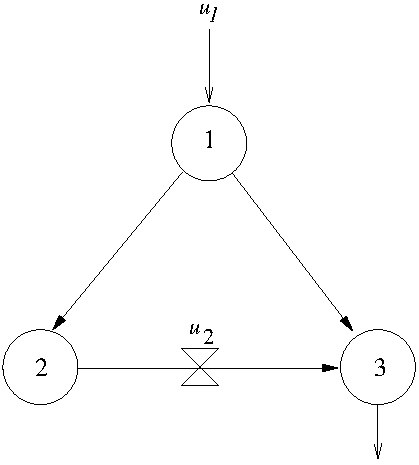
\includegraphics[width=7cm]{graphreseau}
\caption{Vessels network associated graph}
\label{Fig:graphreseau}
\end{center} 
\end{figure}
\cqfd
\end{exemple}
The fundamental structural property of compartments linear systems can be generalized to non linear system with the following theorem.

\begin{theoreme} 
Given a compartments non linear system which flows $q_{ij}$ satisfy C1-C3 conditions.
Therefore, the flows can be written as follows:
\eqnn
&& q_{ij}(x,u) = a_{ij}(x,u)x_i \hspace{4mm}
(i=1,...,n;j=1,...,n)\\ 
&& q_{i0}(x,u) = a_{i0}(x,u)x_i \hspace{4mm}
(i=1,...,n)\\
&& q_{0i} = k_{0i}u_i
\eeqnn
where functions $a_{ij}(x,u)$ et $a_{i0}(x,u)$, defined on the positive orthant, are continuous. 

Therefore, the system state model can be written as:
$$ \dot x = A(x,u)x + Bu $$
where the matrix $A(x,u)$ is a diagonally dominant Metzler matrix for all $(x,u)$ in the positive orthant 
and $B$ an elementary matrix.
\cqfd
\end{theoreme}

We will end this chapter with another industrial classical compartmental system example.

\begin{exemple}{\bf \em Binary distillation process}

A binary distillation process is a process used to split a liquid load composed of two liquid chemical components.
A {\it depropanizer} used to split propane from butane is a typical example of binary distillation process within the petrochemical industry.

The split is made by evaporation in an enclosed vessel called {\em round-bottom flask} (see figure \ref{Fig:distillation}).
\begin{figure}[h]
\begin{center}
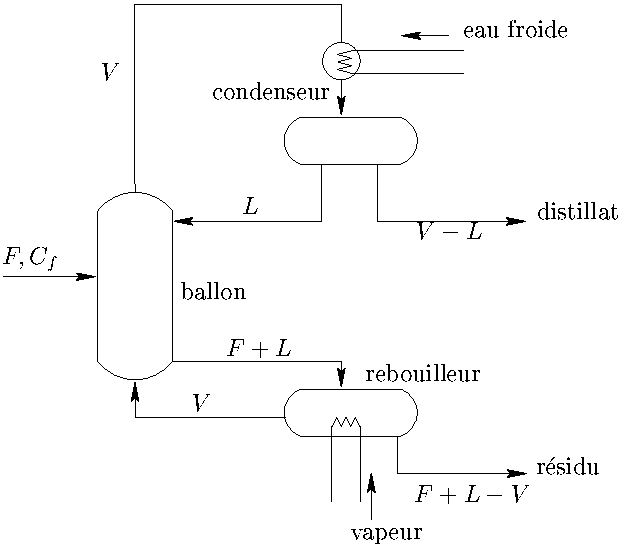
\includegraphics[width=8cm]{proc_distil}
\caption{Distillation process}
\label{Fig:distillation}
\end{center} 
\end{figure}
The {\it distillate} containing mainly the lightest component with a bit of the heaviest one exits from the top of the flask.

The {\it residue} containing mainly the heaviest component with a bit of the lightest one exits from the bottom of the flask.

The flask is filled by the liquid load with a molar debit $F$ (mol/min). 
The steam flow spreading out the flask is cooled down and entirely condensed.
The outgoing liquid is partially recycled toward the flask with a molar debit $L$. 

The remaining part, called {\it distillate}, is extracted from the system.

At the bottom of the flask, the outgoing liquid is warmed up a boiler and the produced steam is recycled within the flask.
The remaining part, called {\it residue}, is extracted from the system.

The distillation process dynamic is simplified by the following modeling assumptions and represented below:
\begin{enumerate}
\item the load is liquid and has the flask temperature;
\item the liquid and steam state in the flask and the boiler are homogeneous and at equilibrium;
\item the flask pressure is constant and there is no steam accumulation; this assumption allows to omit pressure dependencies
in the equations and implies that the steam debit $V$  exiting the flask is equivalent to the input debit; 
\item the liquid extraction debits are adjusted such as the total molar masses of the components in liquid state remain constant : 
the distillate is therefore extracted with a molar debit $V-L$, the liquid at the bottom of the flask is extracted with a molar debit $F+L$
and the residue is extracted with a molar debit $F+L-V$. Obviously, this implies that the inequality $0 < L < V < F+L$ has to be verified.\\
\end{enumerate}

Given this definition, the distillation process can be interpreted as a compartments system which dynamic model is based on
balance equations of one of the two components in the flask, in the condenser and in the boiler.
This compartments system graph is presented on figure \ref{Fig:graphdisti} and the state equations are:
\begin{equation*} \begin{split}
\dot x_1 &= u_2 k(x_2) - u_{1}\frac{x_1}{m_1} - (u_2 - u_1) \frac{x_1}{m_1}\\
\dot x_2 &= u_1\frac{x_1}{m_1} - (u_1+u_3)\frac{x_2}{m_2} + u_2(k(x_3) - k(x_2)) + u_3c_f\\
\dot x_3 &= (u_1 + u_3)(\frac{x_2}{m_2} - \frac{x_3}{m_3}) + u_2(\frac{x_3}{m_3} - k(x_3))
\end{split} \end{equation*}
\begin{figure}[h]
\begin{center}
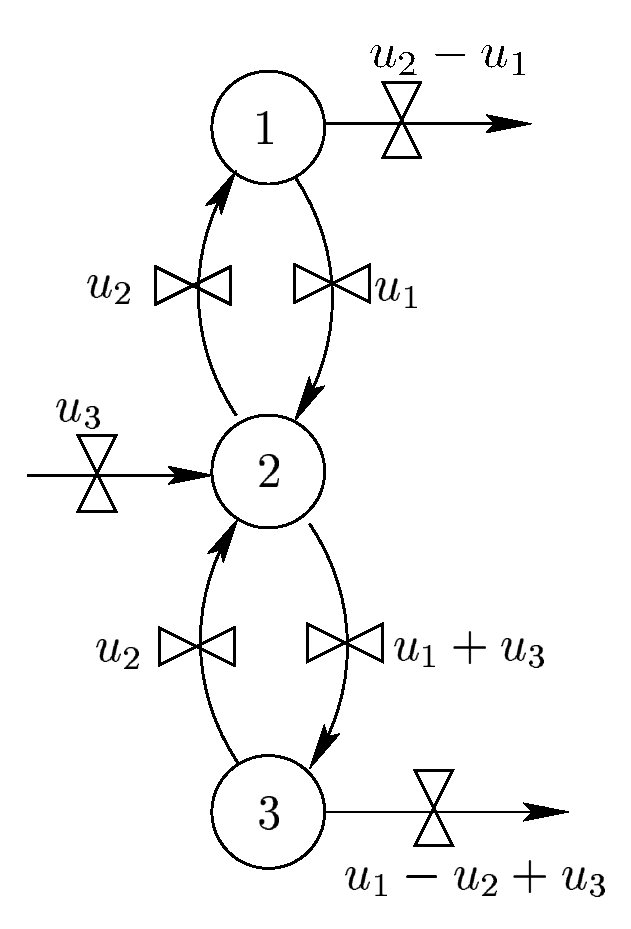
\includegraphics[width=5cm]{graphprocdistil}
\caption{Distillation process associated graph}
\label{Fig:graphdisti}
\end{center} 
\end{figure}
State variables $x_i$ stand for the molar mass of the lightest component in the liquid state within
the condenser (index $1$), the flask (index $2$) and the boiler(index  $3$);

Parameters $m_i$ represent those total (and constant) molar masses : 
the ratio $x_i/m_i$ corresponds to the {\it molar fraction}; 
parameter $c_f$ molar fraction of the lightest component within the load; 

Input variables $u_1 = L$, $u_2 = V$ and $u_3 = F$ are, respectively, molar debit of the reflux, the steam production and the supply.
Finally, the function $k(x)$ is a liquid-steam equilibrium relationship allowing to link the molar fraction of the lightest component
leaving the liquid by vaporization to the molar fraction of the component in liquid state. 
\begin{figure}[ht]
\begin{center}
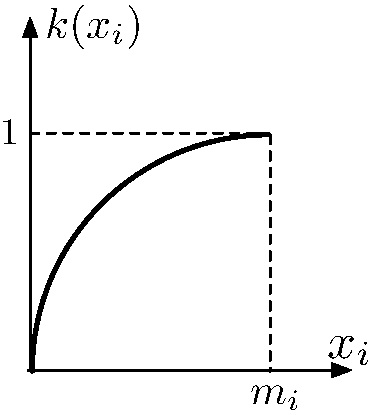
\includegraphics[width=4cm]{separ}
\caption{Liquid-steam equilibrium relationship}
\label{Fig:separ}
\end{center} 
\end{figure}

\noindent This relationship is classically expressed as follows:
\eqnn
k(x_i) \triangleq \frac{\alpha x_i}{m_i + (\alpha - 1)x_i}
\eeqnn
where the constant parameter $\alpha > 1$ is called separation factor.
This function, defined on the interval $[0,m_i]$, checks $k(0) = 0$ and
$k(m_i) = 1$ (see figure \ref{Fig:separ}). \qed  
\end{exemple}

\section{Exercises}

\begin{exercice}{\bf \em A compartments system}

Given the following dynamical system:
\begin{align*}
\dot x_{1} &= x_{3} - \log (1+x_{1}) \\
\dot x_{2} &= x_{3} - x_{2}^2 \\
\dot x_{3} &= x_{2}^2 - 2x_{3} + u
\end{align*}
Demonstrate that it is a compartments system. Draw the associated graph. Compute the flows $q_{ij}$, the matrix $L$ and the matrix $A(x,u)$. \qed
\end{exercice}
\vv

\begin{exercice}{\bf \em A hydraulic system}

A hydraulic system containing three vessels and two pumps is presented on figure \ref{Fig:systhydr}.
\begin{figure}[h]
\begin{center}
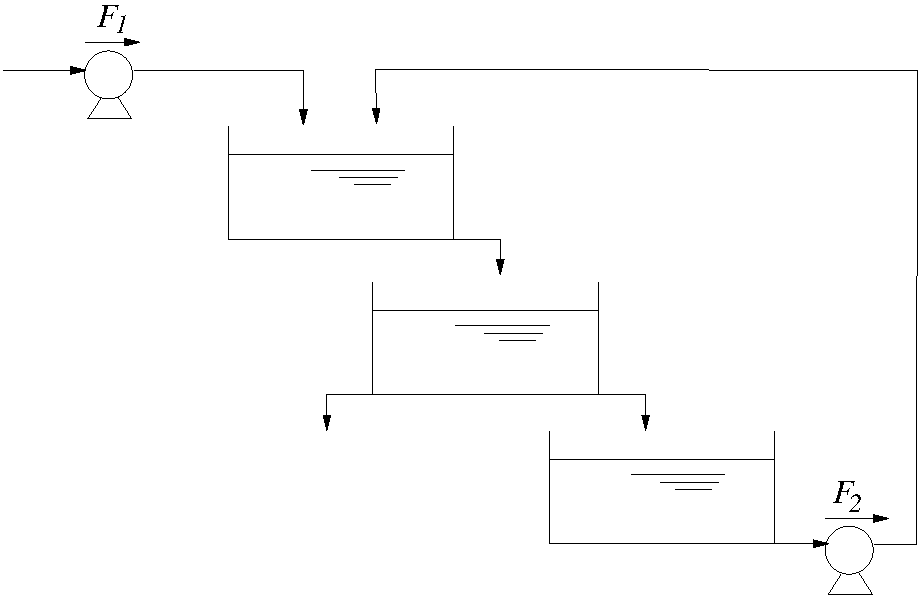
\includegraphics[width=8cm]{systhydr}
\caption{Hydraulic system}
\label{Fig:systhydr}
\end{center} 
\end{figure}
\begin{enumerate}
\item Establish a state model for the system, where the volumetric debits $u_1 = F_1$ and $u_2 = F_2$ are input variables. 
Show that the obtained system is {\it not} a positive system. 
\item Suggest an alternative definition for the input variable $u_2$ which ensure a postive system. 
\item Draw the obtained compartments graph model. \qed
\end{enumerate}
\end{exercice}
\vv 

\begin{figure}[!ht] 
\begin{center}
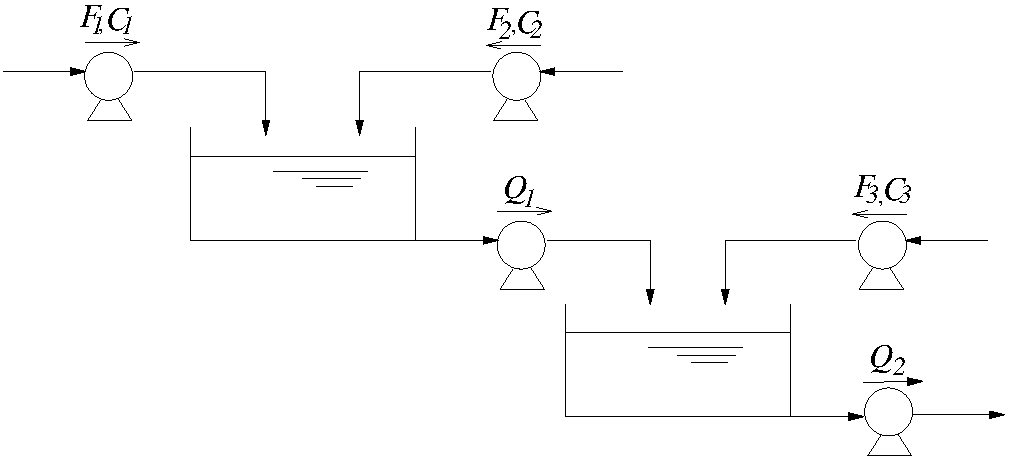
\includegraphics[width=8cm]{cuvmel}
\caption{Mixing vessels network}
\label{Fig:cuvmel}
\end{center} 
\end{figure}

\begin{exercice}{\bf \em A mixing vessels network}

The system represented on figure \ref{Fig:cuvmel} is designed for mixing three substances $X_1, X_2, X_3$ 
whose supply concentrations are denoted $C_1, C_2, C_3$ respectively.

The contained volumes in the two vessels are denoted $V_1$ and $V_2$. 
The pump volumetric debits are denoted as $Q_1, Q_2, F_1, F_2, F_3$.

\begin{enumerate}
\item Establish a state model of the system with the following input variables: 
$u_1 = Q_1/V_1, u_2 = Q_2/V_2, u_3 = C_1, u_4 = C_2, u_5 = C_3$. 
The debits $F_i$, $i = 1, \dots , 3$, are supposed constants.
\item Justify the input variables $u_1$ and $u_2$ form. \qed
\end{enumerate}
\end{exercice}
\vv

\begin{exercice}{\bf \em Compartments linear model}

Characterize the graph structure of a compartments linear model whose associated matrix $A$ is:
\begin{enumerate}
\item bidiagonal
\item tridiagonal
\item lower triangular \qed
\end{enumerate}
\end{exercice}
\vv

\begin{exercice}{\bf \em Distillation process model}

Determine the matrix $A(x,u)$ of the distillation process model. \qed
\end{exercice}
\vv

\begin{exercice}{\bf \em Communicating vessels}

A system with two communicating vessels is represented on figure \ref{Fig:reservoircom}.
The liquid flows freely between the two vessels and towards the outside under the hydrostatic pressure action.

\begin{figure}[h]
\begin{center}
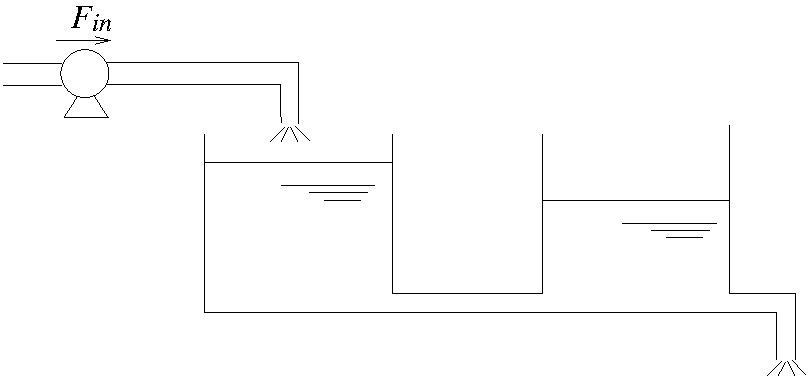
\includegraphics[width=8cm]{reservoircom}
\caption{Communicating vessels}
\label{Fig:reservoircom}
\end{center} 
\end{figure}

\begin{enumerate}
\item Establish a state model of the system. The provided debit (by the supply pump) is the only input variable. 
\item Show that it is a compartments system. Draw the associated graph. Explain the flow between the compartments. \qed
\end{enumerate}
\end{exercice}

\end{document}
